% Template for Cogsci submission with R Markdown

% Stuff changed from original Markdown PLOS Template
\documentclass[10pt, letterpaper]{article}

\usepackage{cogsci}
\usepackage{pslatex}
\usepackage{float}
\usepackage{caption}

% amsmath package, useful for mathematical formulas
\usepackage{amsmath}

% amssymb package, useful for mathematical symbols
\usepackage{amssymb}

% hyperref package, useful for hyperlinks
\usepackage{hyperref}

% graphicx package, useful for including eps and pdf graphics
% include graphics with the command \includegraphics
\usepackage{graphicx}

% Sweave(-like)
\usepackage{fancyvrb}
\DefineVerbatimEnvironment{Sinput}{Verbatim}{fontshape=sl}
\DefineVerbatimEnvironment{Soutput}{Verbatim}{}
\DefineVerbatimEnvironment{Scode}{Verbatim}{fontshape=sl}
\newenvironment{Schunk}{}{}
\DefineVerbatimEnvironment{Code}{Verbatim}{}
\DefineVerbatimEnvironment{CodeInput}{Verbatim}{fontshape=sl}
\DefineVerbatimEnvironment{CodeOutput}{Verbatim}{}
\newenvironment{CodeChunk}{}{}

% cite package, to clean up citations in the main text. Do not remove.
\usepackage{cite}

\usepackage{color}

% Use doublespacing - comment out for single spacing
%\usepackage{setspace}
%\doublespacing


% % Text layout
% \topmargin 0.0cm
% \oddsidemargin 0.5cm
% \evensidemargin 0.5cm
% \textwidth 16cm
% \textheight 21cm

\title{``I won't lie, it wasn't amazing'': Modeling polite indirect speech}


\author{{\large \bf Erica J. Yoon}, {\large \bf Michael Henry Tessler}, {\large \bf Noah D. Goodman} \and {\large \bf Michael C. Frank}  \\
        \{ejyoon, mtessler, ngoodman, mcfrank\} @stanford.edu \\ 
        Department of Psychology, Stanford University}

\begin{document}

\maketitle

\begin{abstract}
Why are we polite when we talk to one another? One hypothesis is that
people expect others to choose what to say based on their goals both to
transfer information efficiently (an epistemic goal) and to make the
listener feel good (a social goal). In our previous work, we found that
when these two goals conflict, they sometimes produce white lies. In the
current work, we expand on this theory to consider another prominent
case of polite speech: indirect remarks using negation (e.g., ``It
wasn't amazing''). With minimal extensions from our previous framework,
our formal model suggests that a pragmatic speaker will produce more
indirect remarks when the speaker wants to be considerate and
informative at the same time. These predictions were borne out in an
experiment on language production. These findings suggest that the
conflict between social and epistemic goals can account for a broad
range of politeness phenomena.

\textbf{Keywords:}
Politeness; computational modeling; communicative goals; pragmatics
\end{abstract}

\definecolor{Red}{RGB}{255,0,0} \definecolor{Green}{RGB}{10,200,100}
\definecolor{Blue}{RGB}{10,100,200} \definecolor{Orange}{RGB}{255,153,0}

\newcommand{\ejy}[1]{\textcolor{Red}{[ejy: #1]}}  
\newcommand{\ndg}[1]{\textcolor{Green}{[ndg: #1]}}  
\newcommand{\mht}[1]{\textcolor{Blue}{[mht: #1]}}  
\newcommand{\mcf}[1]{\textcolor{Orange}{[mcf: #1]}}







\section{Introduction}\label{introduction}

Language users hear and produce \emph{polite speech} on a daily basis.
Adults and even young children spontaneously produce requests in polite
forms (Axia \& Baroni, 1985; Clark \& Schunk, 1980), and speakers use
politeness strategies even while arguing, preventing unnecessary offense
to their interactants (Holtgraves, 1997). But being polite conflicts
with one important goal of cooperative communication: exchanging
information efficiently and accurately (Grice, 1975). People tell white
lies (``Your new dress is gorgeous!'') and produce indirect speech that
is longer and more nuanced than the simplest form of their intended
message (``I don't think that dress looks phenomenal on you'' as opposed
to ``That dress looks terrible'') to make others feel good about
themselves. Speakers risk potential loss of their intended message
(indirect speech), intentionally convey wrong information (lies), and
suffer inefficiencies -- all in the service of being polite. If
information transfer were the only currency in communication, politeness
would be both infelicitous and undesirable.\\

A \emph{cooperative speaker}, however, can be imagined as one who has an
epistemic goal to improve the listener's knowledge state \emph{as well
as} a social goal to minimize any potential damage to the hearer's (and
the speaker's own) self-image, called \emph{face} (Brown \& Levinson,
1987). If the speaker's intended meaning contains no threat to the
speaker or listener's face, then the speaker will choose to convey the
meaning in an explicit and efficient manner (putting it ``on the
record''). As the degree of face-threat becomes more severe, however, a
speaker will choose to be polite by producing more indirect utterances.

Inspired by this set of ideas, we have argued that language users think
about polite speech as reflecting a tradeoff between two goals:
information transfer (which we called \emph{epistemic utility}) and
face-saving (\emph{social utility}; Yoon, Tessler, Goodman, \& Frank,
2016). A speaker with a high weight on social utility will try to save
her listener's face: She hides or risks losing information in her
intended message by making her utterance false or indirect to some
degree. On the other hand, a speaker with a high weight on epistemic
utility prioritizes truthfulness and informativity, and she may risk a
loss of the listener's (or the speaker's own) face. These idaes were
formalized in a model of pragmatic language understanding, building on
the Rational Speech Act (RSA) theory (for a review, see {\textbf{???}}).
We tested the polite RSA model (pRSA) by examining white lies. The model
captured human participants' inferences about a speaker's goals given
her utterance (e.g., saying a \emph{good} talk was ``great'' implies
that she is being nice) and about the world given a speaker's goal
(e.g., saying ``great'' may mean the talk was only \emph{good} or
\emph{ok}). People attributed the goal to be nice increasingly as the
speaker's utterance was more positively biased from the true states, and
inferred worse true states than the literal meaning when the speaker was
described as wanting to be nice.

In the current work, we extend our framework to another polite speech
act: \emph{indirect speech}. White lies are when a speaker tries to save
the listener's face by stretching the truth. But instead of lying,
people sometimes try to be polite by being more indirect. Through
indirect speech, a speaker can express meaning that is different from
the literal meaning of the utterance ({\textbf{???}}). In this work, we
focus on negation (``not''), which has the potential to be indirect. For
instance, ``Mark \emph{isn't} the cleanest person I know'' may suggest
that the speaker thinks Mark is \emph{unclean} (inferred meaning) rather
than not being the person Mark knows who has the greatest degree of
cleanliness (literal meaning). Negation can be used as a hedging or
mitigating device to address an undesirable state that is
face-threatening to the addressee (Brown \& Levinson, 1987; Grice,
1975), and can imply that the intended meaning is worse than the vague
meaning.

What may lead a speaker to produce indirect remarks with negation?
Following our previous work, we hypothesize that if Alice observes Bob's
terrible presentation and says, ``it wasn't amazing'', this reflects her
attempt to balance between epistemic and social goals. Informationally,
``not amazing'' does not preclude the possibility that the presentation
was bad, so the utterance is not a downright lie. And socially, Alice
tries to save Bob's face by not being explicitly critical (e.g., not
saying ``it was terrible''). On the other hand, if the presentation was
actually good, or even decent, Alice will prefer to produce a directly
positive remark (``It was good''). Thus we predict that a speaker who
wants to balance between epistemic and social goals would produce
indirect speech relatively more, especially when the true state is bad.
Importantly, we predict it is the interaction between presence of face
threat (due to addressee's poor performance) and speaker's consideration
of both epistemic and social goals that is predicted to lead to a
greater degree of indirect speech production. In what follows, we derive
our hypotheses using our formal model and present an empirical test of
the hypotheses.

\section{Computational Model}\label{computational-model}

In the current work, we introduce minimal extension to our previous RSA
model (pRSA; Yoon et al., 2016) to allow for speaker production of
indirect remarks using negation.

\subsection{Polite RSA}\label{polite-rsa}

RSA models assume speakers choose utterances approximately optimally
given a utility function (Goodman \& Stuhlmüller, 2013). pRSA posited
that the speaker's utility function can be decomposed into two
components. First, \emph{epistemic utility} (\(U_{epi}\)) refers to the
standard, informative utility in RSA: the amount of information a
\emph{literal listener} (\(L_0\)) would still not know about world state
\(s\) after hearing a speaker's utterance \(w\). Second, \emph{social
utility} (\(U_{soc}\)) is the expected subjective utility of the state
the listener would infer given the utterance \(w\). The expected
subjective utility is related to the intrinsic value of the state, and
we use a value function (\(V\)) to map states to subjective utility
values. This captures the affective consequences for the listener of
being in state \(s\). Finally, some speech acts might be more costly
than others. The utility of an utterance subtracts the cost \(c(w)\)
from the weighted combination of the social and epistemic utilities.

\[U(w;s;  \hat{\beta}) = \beta_{epi}\cdot \ln(P_{L_0}(s \mid w)) 
\\+ \beta_{soc} \cdot \mathbb{E}_{P_{L_0}(s \mid w)}[V(s)]- C(w)\]

The speaker (\(S_1\)) in pRSA chooses utterances \(w\) softmax-optimally
given the state \(s\) and his goal weights \(\hat{\beta}\). The
pragmatic listener (\(L_1\)) jointly infers the state \(s\) and the
utility weights of the speaker, \(\beta_{epi}\) and \(\beta_{soc}\)
(Goodman \& Lassiter, 2015; Kao, Wu, Bergen, \& Goodman, 2014).

\begin{align}
P_{L_1}(s, \hat{\beta} \mid w) &\propto P_{S_1}(w \mid s, \hat{\beta})\cdot P(s) \cdot P( \hat{\beta}) \label{eq:L1}\\
P_{S_1}(w \mid s, \hat{\beta}) &\propto \mathrm{exp}(\lambda_{1} \cdot \mathbb{E}[U(w; s;  \hat{\beta})]) \label{eq:S1}\\
P_{L_0}(s \mid w) &\propto [[w]](s) \cdot P(s) \label{eq:L0}
\end{align}

Within our experimental domain, we assumed there were five possible
states of the world corresponding to the value placed on a particular
referent (e.g., rating deserved by the presentation the speaker is
commenting on, akin to a Yelp rating): \(S = \{s_{1}, ..., s_{5}\}\). We
assume a uniform prior distribution over possible states of the world.
The states have subjective numerical values
\(V(s_{i}) = \alpha \cdot i\), where \(\alpha\) is a free parameter.
\([[w]](s)\) corresponds to the lexical meaning of the utterance \(w\)
(e.g., ``good'') when applied to state \(s\). We gather independent
ratings for these literal meanings.

\subsection{Extensions to pRSA}\label{extensions-to-prsa}

The current work builds on pRSA by adding three simple but key
components to predict indirect remark production.

First, we extend the utterance alternatives to include negation.
Previously we considered five possible utterances: \{It was
\emph{terrible}, \emph{bad}, \emph{okay}, \emph{good}, and
\emph{amazing}\}, all direct assertions of specific states (e.g., ``It
was amazing'' would be true for the state of 5 but untrue for the states
of 1 or 2). Now the speaker may say, \{It \emph{wasn't} terrible, bad,
okay, good, and amazing\}. These utterances indirectly address the
referent by negating certain state.

Second, we assume that it is more costly to say utterances with negation
\mht{cite costly negation}. In our full data analysis, we put a prior on
this cost parameters and infer it's likely values from the data.

Third, we extende the recursive reasoning in the model. For our
experiment, we consider the pragmatic speaker (\(S_2\)) who chooses an
utterance based on the pragmatic listener model (Eq. \ref{eq:L1}),
thinking about the state as well as goal weights that the pragmatic
listener will infer.

\[P_{S_2}(w \mid s, \hat{\beta})\propto \mathrm{exp}(\lambda_{2} \cdot \ln(P_{L_1}(s,  \hat{\beta} \mid w)) - C(w))\]

In addition to these extensions, we simplify from the Yoon et al. (2016)
model by including only a single mixture parameter \(\phi\) governing
the extent to which the speaker is being informative vs.~face saving:
\(\beta_{epi} = \phi\), \(\beta_{soc} = 1 - \phi\).
\mht{note? (or discuss) this parametrization doesn't have "antisocial" goals}.
We implemented this model using the probabilisitic programming language
WebPPL (Goodman \& Stuhlmüller,
2014)\footnote{A complete implementation of the model, links to the experiments, raw data and analyses can be found at \url{https://github.com/ejyoon/cogsci2017}.}.

In the next section, we explore the model's predictions for speaker
productions of indirect speech with negation vs.~direct speech with no
negation.

\section{Schematic model predictions}\label{schematic-model-predictions}

We initially test our hypotheses on a schematic model, with fixed goal
weights and parameters.

\subsection{Semantic measurement}\label{semantic-measurement}

We first probed judgments of literal meanings of the target words
assumed by our model and used in all our experiments. We used these
judgments to set expected literal meanings of utterances in our initial
model predictions, and used them as informative priors to infer literal
meaning for the utterances in the experiment for the model fitting.

\begin{CodeChunk}
\begin{figure*}[t]

{\centering 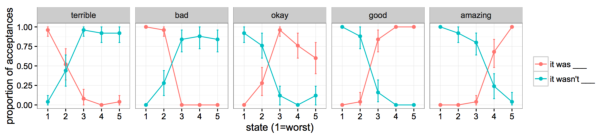
\includegraphics{figs/expt1_results-1} 

}

\caption[Semantic measurement results]{Semantic measurement results. Proportion of acceptances of utterance types (shown in different colors) combined with target words (shown in different facets) given the true state represented on a scale of hearts. Error bars represent 95\% confidence intervals.}\label{fig:expt1_results}
\end{figure*}
\end{CodeChunk}

\begin{CodeChunk}
\begin{figure*}[t]

{\centering \includegraphics{figs/model_pred_negNoneg-1} 

}

\caption[Schematic model predictions (left), experimental results (center) and fitted model predictions (right) for average proportion of negation produced among all utterances, given true states (x-axis) and goals (colors)]{Schematic model predictions (left), experimental results (center) and fitted model predictions (right) for average proportion of negation produced among all utterances, given true states (x-axis) and goals (colors).}\label{fig:model_pred_negNoneg}
\end{figure*}
\end{CodeChunk}

\subsubsection{Materials and methods}\label{materials-and-methods}

\ejy{is it okay to use this way of sectioning?} 25 participants with IP
addresses in the United States were recruited on Amazon's Mechanical
Turk. We used 13 different context items that were previously used in
Yoon et al. (2016), in which someone evaluated a performance of some
kind. For example, in one of the contexts, Bob saw a presentation, and
Bob's feelings toward Ann's cake (\emph{true state}) were shown on a
scale out of five hearts (e.g., two out of five hearts filled in red
color). The question of interest was ``Do you think Bob thought the
presentation was / wasn't X?'' where X could be one of five possible
words: \emph{terrible}, \emph{bad}, \emph{okay}, \emph{good}, and
\emph{amazing}, giving rise to ten different possible utterances (with
negation or no negation). Each participant read 50 scenarios, depicting
every possible combination of 5 true states and 10 utterances.
Participants indicated their answer to each question by answering ``No''
or ``Yes.'' The order of context items was randomized, and there were a
maximum of four repeats of each context item per participant.

\subsubsection{Results}\label{results}

For this and next experiments, we analyze the data by collapsing across
context items. Meanings of the words as judged by participants were as
one would expect (see Figure 1). We used the fraction of participants
that endorsed utterance \(w\) for state \(s\) to set informative priors
to infer posterior credible values of the literal meanings from data in
the speaker production experiment.

\subsection{Model parameters and
predictions}\label{model-parameters-and-predictions}

To model what speakers would say given true states and their goals
(e.g.~wanting to make the listener feel good), we assumed a particular
set of speaker's goal-weights \{\(\beta_{epistemic}\),
\(\beta_{social}\)\} to represent three goal conditions that we are
interested in: \emph{informative} (\(\beta_{epistemic}\) = 0.9;
\(\beta_{social}\) = 0.1); \emph{social} (\(\beta_{epistemic}\) = 0.1;
\(\beta_{social}\) = 0.9); and \emph{both goals} (\(\beta_{epistemic}\)
= 0.5; \(\beta_{social}\) = 0.5). There are four additional parameters
of the model, and for the purposes of generating model predictions a
priori, we will assign reasonable parameters based on pilot runs of the
model-data fit: the speaker optimality parameter (\(\lambda_{S_1}\)
assigned to 2); the pragmatic speaker optimality parameter
(\(\lambda_{S_2}\) to 2); the value scale parameter (\(\alpha\) to 1) in
the utility function; and the cost parameter (\(C(u)\) to 2).

The predictions for the speaker's utterance were consistent with our
hypothesis, namely that indirect speech was relatively more preferred
given bad true states and speaker's consideration of both epistemic and
social goals (Figure 2, left). The model inferred higher likelihood of
negation production for the both-goal condition than informative and
social conditions when the true state was bad (1 heart). For all goal
conditions rate of indirect speech decreased as the true states
improved, also as expected; given a good performance, the speaker should
produce positive direct remarks (e.g. ``It was amazing''). These
simplified predictions thus supported our hypothesis that face threat in
the true state and both epistemic and social utilities contribute to
greater production of indirect speech. Next, we confirm these model
predictions in an experiment.

\section{Speaker production
experiment}\label{speaker-production-experiment}

To compare against our model predictions, we examined people's
predictions for the most likely utterance produced by the speaker
(\(u\)), given a description of the true state of the world (e.g., the
speaker felt that a poem deserved 2 out of 5 hearts) and the speaker's
goals (e.g., the speaker wanted to make the listener feel good).
Critically, the contexts indicated face threats toward the listener, as
the speaker's utterance was an evaluation of the listener's performance.
We hypothesized that when there is no tradeoff between informativity and
face-threat avoidance (i.e.~when the addressee's performance is great),
speakers should use truthful and face-saving direct remarks (``{[}Your
talk{]} was amazing'') regardless of their described goals. However,
when there is a conflict between the epistemic and social goals
(i.e.~when the addressee's performance is poor), a speaker who tries to
compromise between both goals would use vague indirect remarks more
often than direct face-threatening remarks (blunt truth; preferred by an
informative speaker) or direct face-saving remarks (i.e.~white lies;
preferred by face-saving speaker). Our hypothesis and method were
pre-registered prior to data collection on the Open Science Framework
(\url{http://osf.io/b73dm}).

\subsection{Method}\label{method}

\subsubsection{Participants}\label{participants}

202 participants with IP addresses in the United States were recruited
on Amazon's Mechanical Turk.

\subsubsection{Stimuli and Design}\label{stimuli-and-design}

We designed scenarios in which a person (e.g., Ann) gave some
performance and asked for another person (e.g., Bob)'s opinion on the
performance. The same context items and true states as Experiment 1 were
used. Additionally, we provided information on the speaker Bob's goal
(\emph{to make Ann feel good}, or \emph{to give as accurate and
informative feedback as possible}, or both) and the true state, or how
Bob actually felt Ann's performance (e.g., 2 out of 5 hearts), Then we
asked participants to predict what Bob would say, out of 10 possible
utterances (``It was terrible'', ``It was bad'' \ldots{} ``It wasn't
good'', ``It wasn't amazing''). Each participant read 15 scenarios,
depicting every possible combination of 3 goals and 5 states. The order
of context items was randomized, and there were a maximum of two repeats
of each context item per participant.

\begin{CodeChunk}
\captionsetup{width=0.8\textwidth}\begin{figure}[H]

{\centering 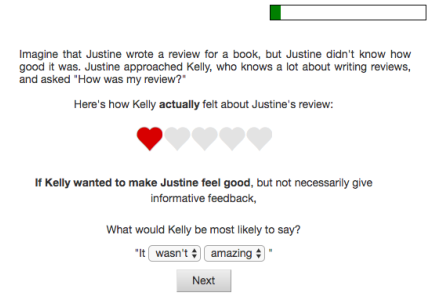
\includegraphics{figs/expt2_screen-1} 

}

\caption[Example of a trial in Experiment 1]{Example of a trial in Experiment 1.}\label{fig:expt2_screen}
\end{figure}
\end{CodeChunk}

\subsubsection{Procedure}\label{procedure}

Participants read each scenario followed by a question that read, ``If
Bob wanted \emph{to make Ann feel good} (or \emph{to give accurate and
informative feedback}, or \emph{BOTH make Sarah feel good AND give
accurate and informative feedback}), what would Bob be most likely to
say?'' Participants indicated their answer by choosing one of the
options on the two dropdown menus, side-by-side, one for choosing
between \emph{was} vs. \emph{wasn't} and the other for choosing among
\emph{terrible}, \emph{bad}, \emph{okay}, \emph{good}, and
\emph{amazing} (see Figure 3).

\subsection{Behavioral results}\label{behavioral-results}

\begin{CodeChunk}
\begin{figure*}[t]

{\centering 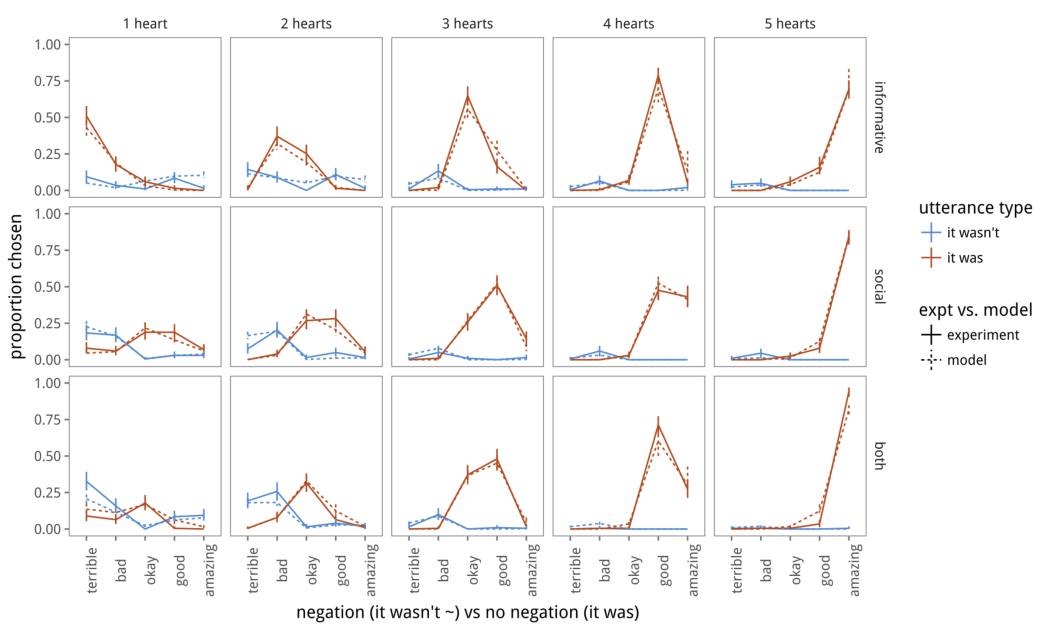
\includegraphics{figs/expt2_results-1} 

}

\caption[Experimental results ("experiment" rows) and model predictions ("model" rows) for speaker production]{Experimental results ("experiment" rows) and model predictions ("model" rows) for speaker production. Proportion of utterances chosen (utterance type -- direct vs. indirect -- on x-axis and words shown in different colors) given the true state (columns) and speaker goals (rows). Error bars represent 95\% confidence intervals for the data and 95\% highest density intervals for the model.}\label{fig:expt2_results}
\end{figure*}
\end{CodeChunk}

Our hypotheses for utterance production by speakers with different goals
were borne out: People's predictions for speaker's use of indirect
vs.~direct remarks given varied depending on speaker's goals, and these
differences were especially pronounced for worse true states (Figure 3,
center). Predictions for individual utterances were also intuitive. For
good states (4 and 5 hearts), positive direct remarks were judged to be
the most likely utterances across all three goal conditions. For
less-than-perfect, but still decent states, there was a greater degree
of expectation of white lies (e.g., ``It was amazing'' for 4 hearts)
given social goal (Figure 4, right). For bad states (1 and 2 hearts), as
we predicted, there were more instances of expected indirect remarks
overall across all goal conditions given bad states. Critically,
speakers with both goals to be informative and socially considerate
produced more indirect than direct remarks, unlike the other two goal
conditions. Thus, these results indicated that a speaker who considers
both informative and social goals, and thus is in want of a compromise
between the two, is expected to produce relatively more indirect
remarks.

\subsection{Model predictions}\label{model-predictions}

\subsubsection{Model fitting}\label{model-fitting}

In this experiment, participants were told true states and what
speakers' intentions were (e.g., Bob wanted to make Alice feel good). We
assume that the intention descriptions conveyed to the participants a
particular set of goal-weights \{\(\beta_{epi}\), \(\beta_{soc}\)\} that
the speaker was using. We put uninformative priors on these weights
(\(\beta\) \textasciitilde{} Uniform(0,1)) and infer their credible
values separately for each goal condition (``wanted to X'') using
Bayesian data analytic techniques (Lee \& Wagenmakers, 2014).

There were four additional parameters of the model: the speaker
optimality parameter (\(\lambda_{S_1}\)); the pragmatic speaker
optimality parameter (\(\lambda_{S_2}\)); the value scale parameter
(\(\alpha\)) in the utility function; and the cost parameter (\(C(u)\)).
We put uninformative priors on these (\(\lambda_{S_1}\)
\textasciitilde{} Uniform(0,20); \(\lambda_{S_2}\) \textasciitilde{}
Uniform(0,5); \(\alpha\) \textasciitilde{} Uniform(0,5); \(C(w)\)
\textasciitilde{} Uniform(1,10)) and infer their posterior credible
values from the data. We ran 4 MCMC chains for 80,000 iterations,
discarding the first 40,000 for burnin. The Maximum A-Posteriori (MAP)
estimate and 95\% Highest Probability Density Interval (HDI) for
\(\lambda_{S_1}\) are 2.16 {[}2.02, 3.61{]}; for \(\lambda_{S_2}\) 0.91
{[}0.83, 1.75{]}; for \(\alpha\) 2.71 {[}0.98, 4.59{]}; and for \(C(w)\)
2.04 {[}1.95, 2.25{]}. To generate utterance predictions, given our
cognitive model and the inferred parameters, we evaluated the posterior
predictive distribution, marginalizing out all parameters.

\subsubsection{Results}\label{results-1}

The inferred weights for each goal condition were largely as expected:
For the ``wanted to give informative feedback'' (\emph{informative})
condition, the model puts a moderate weight on epistemic utility (0.81).
For the ``wanted to make {[}the listener{]} feel good'' (\emph{social})
condition, the model infers the speaker was using a moderate weight on
epistemic utility (0.51). For the ``wanted BOTH to make {[}the
listener{]} feel good and give informative feedback'' (\emph{both})
condition, the model assigned a weight on epistemic utility between the
weights for the other two goal conditions (0.57). Overall, the weights
tended to be more biased towards prioritizing the epistemic utility.

The predictions for the speaker's utterance were broadly consistent with
experimental findings (Figure 4). The model successfully predicted
distinct patterns for each goal condition. The \emph{informative}
speaker produced direct remarks whose literal meanings mapped onto the
true states (e.g. ``It was terrible'' given 1 heart). The \emph{social}
speaker produced remarks that were positively biased compared to the
true states (e.g. ``It was okay'' given 2 hearts). The \emph{both-goal}
speaker generally produced more indirect remarks with negation than
others (``It was terrible'' had the highest likelihood given 1 heart).

However, the model predictions fit to data did not predict the expected
difference for negation production between both-goal versus informative
and social conditions (Figure 2, right). There are several possible
causes for this finding: the social speaker was inferred to place a
higher weight on epistemic utility in the experimental data compared to
the schematic predictions we used. Thus, the particular goal
descriptions we used in the experiment may have suggested the social
speaker as being equivalently informative as the both-goal speaker. If
this were the case, our argument still holds: a balance between
epistemic and social utility, rather than bias toward one utility over
the other, is what predicts indirect speech production. Another possible
cause is that participants preferred different kind of indirect speech
than the model -- the both-goal speaker preferred to produce ``It wasn't
amazing'' in the schematic predictions of the model, whereas
participants in our experiment chose ``It wasn't terrible'' as the most
likely utterance produced by the both-goal speaker. This discrepancy
between the two remarks is interesting to note, because their implied
meaning is similar; in a task of true-state inference (not reported in
this paper), participants judged the implied state for ``It wasn't
amazing'' and ``It wasn't terrible'' to be similar (\textasciitilde{}2
hearts). What causes this difference in preference for one remark over
the other is a remaining question to be explored.

Overall, however, the expected values of the model explain almost all of
the variance in the average data \(r^2\)(15) = 0.962 (Figure 5). Thus,
the model predictions supported our hypothesis that face threat in the
true state and both epistemic and social utilities contribute to greater
production of indirect speech.

\begin{CodeChunk}
\begin{figure}[h]

{\centering \includegraphics{figs/expt2_model-1} 

}

\caption[Full distribution of human responses vs]{Full distribution of human responses vs. model predictions. Error bars represent 95\% confidence intervals for the data and 95\% highest density intervals for the model.}\label{fig:expt2_model}
\end{figure}
\end{CodeChunk}

\section{Discussion}\label{discussion}

In this work, we showed that our formal model with two speaker utilities
(epistemic and social) can be used to not only explain white lie
understanding but also indirect remark production and comprehension. Our
model on its own predicted that speakers produce more indirect remarks
given poorer performance of the addressee (thus involve greater face
threat) and speaker's goal to both be informative and to save face, and
experimental data confirmed these predictions. Model fit to the data was
very strong, although it did not show the predicted dominance of
indirect speech for both-goal speaker at low states. Whether this
discrepancy between the initial and data-fitted predictions is due to
variation in goal weight based on experimental scenarios, or due to
discrepancy in particular indirect speech preferred by participants
vs.~the model, remains to be answered.

An important contribution of this work is in showing the
generalizability of our formal model to different kinds of polite speech
(white lies and indirect remarks). Can the model be extended to other
polite speech phenomena? One significant factor to take into account
will be speaker's self-presentation: Not only will a speaker want to
save the listener's face, but she also will want to save her own face.
Thus, examining how our model's utilities can be extended to speaker's
desire to save her own face by appearing polite, genuine, or modest will
be an important next step. Using the model to explore other kinds of
polite speech such as indirect requests (``Would you mind closing the
window?''; Clark \& Schunk, 1980), agreeable self-presentations
(e.g.~modesty; ``I didn't do too well on my test''), and manifestations
of polite speech in different cultures (e.g., {\textbf{???}}) will also
be important directions for future research.

In sum, our formal model and experimental work present a key
contribution to polite speech understanding. With a minimal extension to
our existing model, we were able to capture subtle patterns in people's
inferences for indirect speech production. Through empirical findings
compared against our model predictions on indirect speech, we showed
that neither epistemic nor social motives alone motivate indirect
speech; instead, the need for indirect speech results from the conflict
between these two. These findings provide strong support for our
utility-theoretic framing of politeness, and promises next concrete
steps in pragmatic understanding.

\section{Acknowledgments}\label{acknowledgments}

This work was supported by NSF grant BCS \#1456077 to MCF, ONR grant
N00014-13-1-0788 and a James S. McDonnell Foundation Scholar Award to
NDG, NSF Graduate Research Fellowship DGE-114747 to MHT, and NSERC
post-graduate doctoral scholarship PGSD3-454094-2014 to EJY.

\section{References}\label{references}

\setlength{\parindent}{-0.1in} \setlength{\leftskip}{0.125in} \noindent

\hypertarget{refs}{}
\hypertarget{ref-axia1985}{}
Axia, G., \& Baroni, M. R. (1985). Linguistic politeness at different
age levels. \emph{Child Development}, 918--927.

\hypertarget{ref-Brown1987}{}
Brown, P., \& Levinson, S. C. (1987). \emph{Politeness: Some universals
in language usage} (Vol. 4). Cambridge Univ. Press.

\hypertarget{ref-clark1980}{}
Clark, H. H., \& Schunk, D. H. (1980). Polite responses to polite
requests. \emph{Cognition}, \emph{8}(2), 111--143.

\hypertarget{ref-GoodmanLassiter2015}{}
Goodman, N. D., \& Lassiter, D. (2015). Probabilistic semantics and
pragmatics: Uncertainty in language and thought. In S. Lappin \& C. Fox
(Eds.), \emph{The handbook of contemporary semantic theory, 2nd
edition}. Wiley-Blackwell.

\hypertarget{ref-Goodman2013}{}
Goodman, N. D., \& Stuhlmüller, A. (2013). Knowledge and implicature:
Modeling language understanding as social cognition. \emph{Topics in
Cognitive Science}, \emph{5}.

\hypertarget{ref-dippl}{}
Goodman, N. D., \& Stuhlmüller, A. (2014). The Design and Implementation
of Probabilistic Programming Languages. \url{http://dippl.org}.

\hypertarget{ref-Grice1975}{}
Grice, H. P. (1975). Logic and conversation. In \emph{Readings in
language and mind}. Blackwell.

\hypertarget{ref-holtgraves1997}{}
Holtgraves, T. (1997). YES, but. positive politeness in conversation
arguments. \emph{Journal of Language and Social Psychology},
\emph{16}(2), 222--239.

\hypertarget{ref-Kao2014}{}
Kao, J. T., Wu, J. Y., Bergen, L., \& Goodman, N. D. (2014). Nonliteral
understanding of number words. \emph{Proceedings of the National Academy
of Sciences}, \emph{111}(33), 12002--12007.

\hypertarget{ref-LW2014}{}
Lee, M. D., \& Wagenmakers, E. J. (2014). \emph{Bayesian cognitive
modeling: A practical course}. Cambridge Univ. Press.

\hypertarget{ref-yoon2016}{}
Yoon, E. J., Tessler, M. H., Goodman, N. D., \& Frank, M. C. (2016).
Talking with tact: Polite language as a balance between kindness and
informativity. In \emph{Proceedings of the thirty-eighth annual
conference of the Cognitive Science Society}.

\end{document}
